\chapter{Literature Survey} \label{lit}

Systematic reviews have many different stages that propose themselves as a candidate for automation. This section is going to look at the techniques that have been applied for some of these stages in previous literature.


\section{Steps of a Systematic Review}

It is useful for us to break down the steps involved in creating a systematic review into subtasks. This way we can observe what techniques can be applied during the relevant sub tasks to improve the efficiency of the process. The following definitions are derived task simplifactions from the cochrane tutorial on systematic reviews: \cite{cochranes}.

\begin{enumerate}
  \item Question definition.
  \item Relevant literature search.
  \item Data Filtering.
  \item Data Extraction.
  \item Analysis and Data combination.
\end{enumerate}

\subsection{Question Definition}

One of the best known techniques for formulating a systematic review question is known as the PICO strategy \cite{pico}. This technique focuses on exposing 4 pieces of information in the systematic review question: patient population, intervention or exposure, comparison or control and outcome.

Example: (credit goes to \cite{pico})

"Is animal-assisted therapy more effective than music therapy in managing aggressive behaviour in elderly people with dementia?"

\begin{center}
\begin{tabular}{ |c|c| } 
 \hline
 P & elderly patients with dementia \\ 
 I & animal-assisted therapy \\ 
 C & music therapy \\ 
 O & aggressive behaviour \\ 
 \hline
\end{tabular}
\end{center}

A potential point of interest would be attempting to generate these questions automatically given some literature context.

\subsection{Relevant literature search}

After formulating a question, systematic reviews need to search for the relevant literature that surrounds this question.

Large medical database-such as Pubmed \cite{pubmed} contain relevant studies that can be used to create the review. These databases are typically very large and require concise queries to efficiently retrieve data.

Naturally this can be modelled as an information retrieval problem. We have a large number of documents and we wish to retrieve the most relevant ones. One task for the 2017 CLEF conference was to produce a ranking of the most relevant documents for topics \cite{Kanoulas12017}. Many techniques have been proposed for ranking of relevant documents, with varying degrees of performance \cite{Alharbi2017} \cite{Gordon2017} \cite{Eunkyung2017}.

An important aspect of the relevant literature search step is the construction of the query. Query creators often apply filters (also known as hedges) to increase the effectiveness or/and the efficiency of the searching. Two key attributes for the query are the precision and the sensitivity (aka recall). By including synonymous phrases e.g: quality adjusted life or quality of well-being or disability adjusted life the sensitivity can be increased, but as expense of the precision. The creation of this query is a task that could potentially have some aspects of NLP applied to it.


\subsection{Data Filtering}

The data filter stage involves reducing the amount of documents returned by the initial query down to a smaller subset of relevant document. This is can also be referred to as the abstract screening phrase \cite{Kanoulas12017}.

The length of this stage is highly dependant on how many documents were returned by the initial query, often in the excess of 5000 studies for a single query. In response to this, stopping criteria methods have been proposed that aim to optimize two key parameters; the effort and the recall. That is to say we want to get as many relevant documents as possible, whilst looking at the fewest. Examples of approaches include the knee method \cite{Satopa11} and the target method \cite{Cormack2016}. Other techniques could be applied and evaluated such as curve fitting.

\subsection{Data Extraction}

The data extraction phase involves pulling the relevant information from the filtered subset of studies. Examples of important information includes how many people took part in the study and what the results were.

Being able to extract the relevant information from studies presents itself as an information extraction problem. The task to automate the process of extracting relevant information would reduce time and complexities of manually reviewing studies \cite{Siddhartha2015}.


\section{Indexing and Querying Medline and Automated Query Generation}

Medline is a large collection of medical literature and data from around the world. Typically each entity will contain a title and an abstract containing some information on the study. Whilest Medline as a whole is very easy to access \cite{medline}, the large size and complexity of the data makes it difficult to retrieve the relevant information.

Being able to create a reliant index of Medline would help with the effectiveness of the queries. As such existing medline indexes and IR systems have been created \cite{nlm}.

\subsection{Automated Query Generation}

Being able to automate query generation for literature searching would save systematic reviewers a significant amount of time. However, medical literature queries are typically complex and contain multiple levels of logical operators and synonymous term look ups. This makes the task of creating a query manually in-its-self a challenging piece of work.

\subsubsection{Rapid Automatic Keyword Extraction Algorithm}

Rapid automatic keyword extraction (RAKE) is a keyword extraction algorithm was proposed by Rose, Engel and Cramer in 2010 \cite{rake}. This algorithm is used for taking the key pieces of information from text and is useful the domain of information extraction. This algorithm is of interest to us as it has potential usage within the field of query generation.

RAKE heavily relies on stop-words and punctuation separators as an indicator for the importance of a phrases and words. RAKE will iterator over sequences of words until a stop-word or separator is found, this phrase/word is then split and extracted. Frequency of occurrence (tf) and word co-occurrence matrices can then be used to reduce the key-word set down further.

RAKE can be further optimized by specifying minimum term frequency rates to capture more prominent terms.


\section{Stopping Criteria} \label{stops}

Stopping criteria is about finding the optimum point in a set of documents. This could be useful in a decision making process. Consider having 100 relevant documents, where each document contains a binary value. If we looked at 1/3 of these documents and saw a trend of positive values, we could use this to infer the reliability of the remaining documents.

Another use of stopping criteria is when filtering through potentially relevant documents. Consider a query that returns 10000 documents, of which only a small sub-set of these are relevant. Reviewers would need to filter through each of these 10000 documents to pull out the relevant ones. Or it could be that the reviewers are happy to hit a 90\% recall of relevant documents, and are happy to miss the remaining 10\% in exchange for time-saved.

Two key methods have been proposed for finding stopping points so far, the target method \cite{Satopa11} and the knee method. \cite{Cormack2016}. Both these methods are discussed below \ref{methods}


\subsection{Evaluation Metrics for Finding Stopping Points} \label{evalsstops}

In order to evaluate the suitability of our stopping method, we can use two evaluation metrics. The recall, which is simply the number of documents returned for a topic, and effort which is the number of documents we had to look at for a topic. 

\begin{equation}
Recall = \frac{R}{|D|}
\end{equation}

Where $R$ is the number of returned relevant documents and $D$ is the set of all relevant documents.

\begin{equation}
Effort = \frac{L}{|D|}
\end{equation}

Where $L$ is the number of returned documents looked at.

Naturally we could exclusively optimized each of the parameters by either returning everything in the document collection ($R$ = $|D|$) or by just looking at a single document. ($L$ = 1)

Therefore it becomes difficult for us to evaluate our stopping criteria as we need to consider both of these parameters adjacently.

In response to this we can make use of two more evaluation metrics that were proposed by Cormack and Grossman \cite{Cormack2016}:

\begin{equation}
reliability = P [acceptable(S) == 1]
\end{equation}

reliability is computed over all searches and is read as the probability of the acceptability being 1. Where acceptability is calculated as:

\begin{equation}
  acceptability(S)=\begin{cases}
    1, & \text{$recall(S)>=0.7$}.\\
    0, & \text{$recall(S)<0.7$}.
  \end{cases}
\end{equation}

A stopping point is deemed to be acceptable if 70\% of the relevant documents have been found. As such, the reliability is an average over a search method.


\subsection{Existing Stopping Methods} \label{methods}

There are different approaches can be experimented with in finding an optimum stopping point.  Consider a percentage cut-off method, where we use the score similarity score for deciding if its worth continuing to look down the rankings:

\begin{equation}
	  Difference(D_i, D_i+1) > C
\end{equation}

Where difference returns a score of how close document $D_i$ and $D_i+1$ are together and $C$ is a cut-off constant. We can expand this to an example:

\begin{equation}
	  (1 -(0.73 / 0.75)) * 100 > 0.015
\end{equation}

Here we are saying if the two documents' scores are above 1.5\% then we should stop looking down the rankings.

We a basis of how stopping methods work, we can move on to more established and defined methods.


\subsubsection{Target} \label{target}

The target method is an approach that can guarantee a certain a certain level of reliability \ref{evalsstops}. It was first proposed by Cormack and Grossman \cite{Cormack2016}.

The target $T$ denotes how many documents we should randomly select from our initial query. A larger value of $T$ will increase the effort required as we are more likely to select a document towards the end of the query set. Documents are looked at until the target point $T$ has been reached.

We first compute a random target set of relevant documents. We then calculate the last document in the target set and mark that as our target point:

\begin{equation}
	  \underset{last}{d} = \underset{d \in{T}}{argmax relrank(d)}
\end{equation}

It must hold that $d$ is in the target set.

\begin{figure}[H]
\center
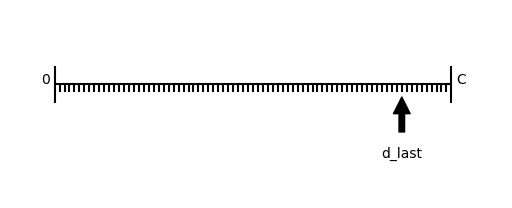
\includegraphics[width=13cm]{figures/target_method.png}
\caption{Visualisation of target method last relevant document selection. $C$ is number of documents in collection.}
\end{figure}

Increasing our target set size is likely to increase the probability the last document being towards the end of the document collection.

We can calculate the recall of the point by looking at the relevance rank of the last document:

\begin{equation}
	  recall = \frac{relrank(\underset{last}{d})}{R}
\end{equation}

Where $R$ is the number of relevant documents.


For our method to be deemed reliable we must achieve 70\% recall with a 95\% average over all topics.

\begin{equation}
	  P(\frac{relrank(\underset{last}{d})}{R} \geqslant 0.7) \geqslant 0.95
\end{equation}




While this approach is shown to acquire 95\% reliability, the effort needed is often significantly highly, often requiring us to look at huge volume of documents.

\subsubsection{Knee Method}

A different stopping kethod proposed by \cite{Satopa11} is known as the knee method. This approach uses a curve to generate a 'knee', which is then used for predicting a stopping point. This approach is likely to be highly dependant on the quality of the initial rankings. This is because we need a curve that reaches a peak quickly, before flattening out.

We use a vertical line panning the length of the ranking set and use it to calculate the distance from the ranking at each point. The point with the maximum distance is chosen as a suitable stopping point.

\begin{figure}[H]
\center
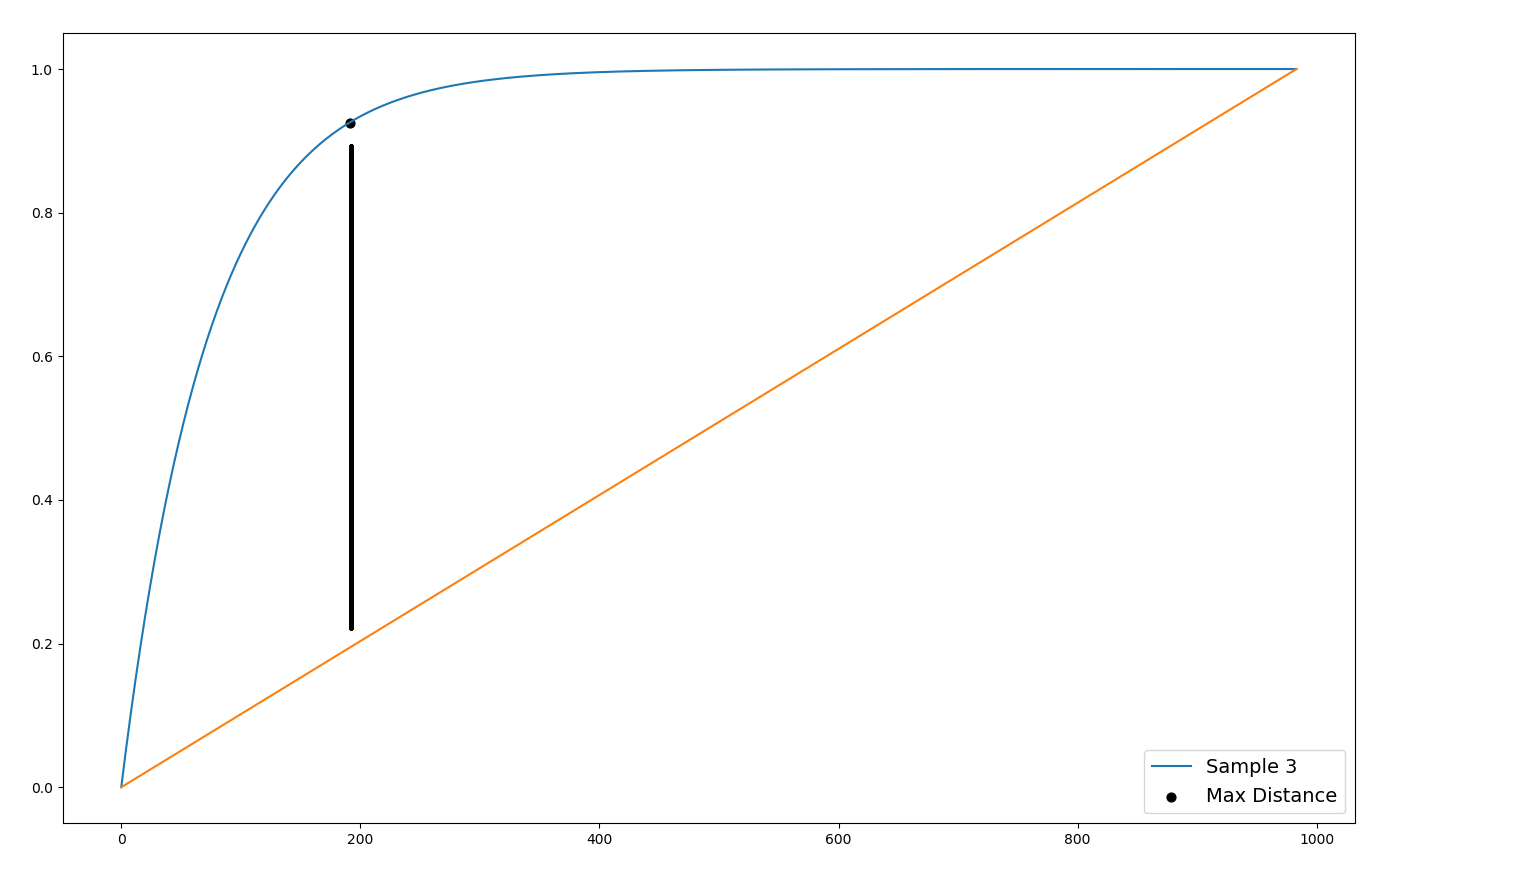
\includegraphics[width=13cm]{figures/knee.png}
\caption{Example of using knee method to find a stopping point. Image inspired from \cite{Satopa11}}
\end{figure}

We can see in the above example the method has predicted we look at around 200 of the 1000 documents to achieve a suitable stopping point.

This method also imposes an additional constraint for rankings of a large volume. 

It was found that the knee method is a better approach for finding a stopping point than the Target method \cite{Cormack2016}. The recall was always found to be better and the reliability was found to be the same or higher for 6 out 8 of the test collections.




